\chapter{引言}
\label{chap01}
\section{机器学习简介}
机器学习\cite{mitchell2007machine}是一种基于数据和统计学的人工智能方法,旨在自动从数据中提取规律和模式,并基于这些规律和模式进行预测和决策。与传统的编程方式不同,机器学习的程序不需要明确规定所有的规则和逻辑,而是通过学习和建模来自动提取规律和模式,从而处理大量复杂的数据,甚至能够发现人类无法感知的模式和规律\cite{李航2012统计学习方法}。

机器学习包括多种算法和技术,例如监督学习、无监督学习和强化学习。在监督学习中,机器学习算法从标记好的数据中学习,以预测未来的输出结果。在无监督学习中,机器学习算法自主从数据中发现结构和模式,而不需要任何标记好的数据。在强化学习中,机器学习算法通过与环境交互,学习最优策略,以达成某种目标。

% 机器学习在图像识别中可以通过训练模型识别出图片中的物体、人脸等信息;在信用评估中可以通过分析用户历史数据预测其信用风险;在金融风险管理中可以对市场数据进行分析预测投资风险;在医疗诊断中可以通过模型学习预测疾病风险或判断疾病种类。
机器学习在各个领域都得到了广泛应用,例如在自然语言处理\cite{chowdhary2020natural}领域,机器学习可以通过学习大量文本数据,自动分析文本中的语法和语义,从而实现文本分类和命名实体识别\cite{刘浏2018命名实体识别研究综述}等任务;
在图像识别领域,机器学习可以通过训练模型识别出图片中的物体、人脸等信息;
在信用评估中可以通过分析用户历史数据预测其信用风险;
在金融风险管理中可以对市场数据进行分析预测投资风险;在医疗诊断中可以通过模型学习预测疾病风险或判断疾病种类。
在这些领域中,机器学习可以通过从大量数据中学习和发现模式,提高预测准确性和效率,甚至超过人类的表现。

因此,机器学习是一种基于数据和统计学的人工智能方法,通过不断学习和优化,让计算机可以自主完成某些任务和决策,具有广泛的应用前景。

\section{中子共振数据简介}
% 当用低能中子去轰击靶核并测量其激发曲线时,会看到曲线的形状出现许多宽窄不等、高低不齐的共振峰,每个峰的最高点所对应的激发能通常被称为共振能量或共振能级,每个峰所对应的半宽度为共振宽度。共振截面、共振能量和共振宽度是描述中子共振现象的几个最基本物理量。
% 实验表明:除氕、氘、氚以外的所有核素均存在中子共振现象,但不同核素的共振谱各不相同,每种核素都有其独一无二的中子共振谱。中子共振截面具有几大鲜明的特征[1]:①特定核素的峰值出现在特定的能量下,这一性质为同位素识别、同位素定量测量以及它们衍生的各类核探测技术提供了强有力的支撑。②中子共振截面非常大,常常高于快中子能区几个数量级,这在实际应用中非常重要并产生极大的影响。③中子共振截面不受压力、温度、湿度、形状、大小等物质形态的影响。中子共振截面因具备上述特性,可应用于多种极端条件,如炸药爆轰或冲击波等动态系统中最难测量的瞬时温度;无损检测极其珍贵稀缺文物、航空发动机、涡轮叶片等特定核素的含量和分布;核反应堆中铀富集度检测或二氧化钚分布检测;发生融堆核事故后核燃料形态和新核素形成检测等。[1]	庹先国, 刘福乐, 王琦标, 等. 中重核中子共振研究及应用进展. 核技术, 2020, 43(10): 100201.


% 中子共振数据在新一代核能技术、核天体物理、基础核物理学、核医学和国防战略武器研究\cite{郭之虞2003核技术及其应用的发展}中起着重要作用。
% 当中子与原子核发生相互作用时,有多种物理过程,如吸收、散射和发射,其中中子诱导的核反应是指中子与原子核相互作用后,产生多种变化,如中子的弹性散射和辐射俘获,同时释放出能量的反应。核反应在核能和核医学等领域有广泛应用\cite{glasstone2012nuclear},例如核电站发电、放射性同位素制备、医疗诊断和治疗等。
中子核反应的基本过程包括中子的入射、原子核的吸收和复合核的形成,以及复合核的衰变等多个阶段\cite{卢希庭2000原子核物理}。中子与原子核相互作用的方式取决于中子的能量和原子核的结构。当中子的能量较低时,会与原子核中的核子发生相互作用,导致原子核激发或熔合。而当中子的能量足够高时,原子核会发生裂变等其他核反应。
在核物理学中,截面(Cross section)是衡量原子核反应中发生特定相互作用的可能性大小的物理量,截面越大,发生某特定核反应的概率也就越大。截面通常会随着中子能量的变化而变化,
% 并在一定能量范围内产生共振结构。共振结构指的是,在一定能量范围内,中子与原子核相互作用的截面呈现出明显的尖峰状,这种尖峰结构被称为共振峰,共振峰对应的截面称为共振截面。
当用低能中子去轰击靶核并测量其激发曲线时,会出现曲线的形状出现许多宽窄不等、高低不齐的共振峰,共振峰对应的截面称为共振截面。以$^{235}\text{U}(n,f)$反应为例,此反应的实验数据数据如图\ref{u235expendf}所示。从图中分析得到,在高频共振区有900多个共振峰。
\begin{figure}[htbp!]
  \centering
  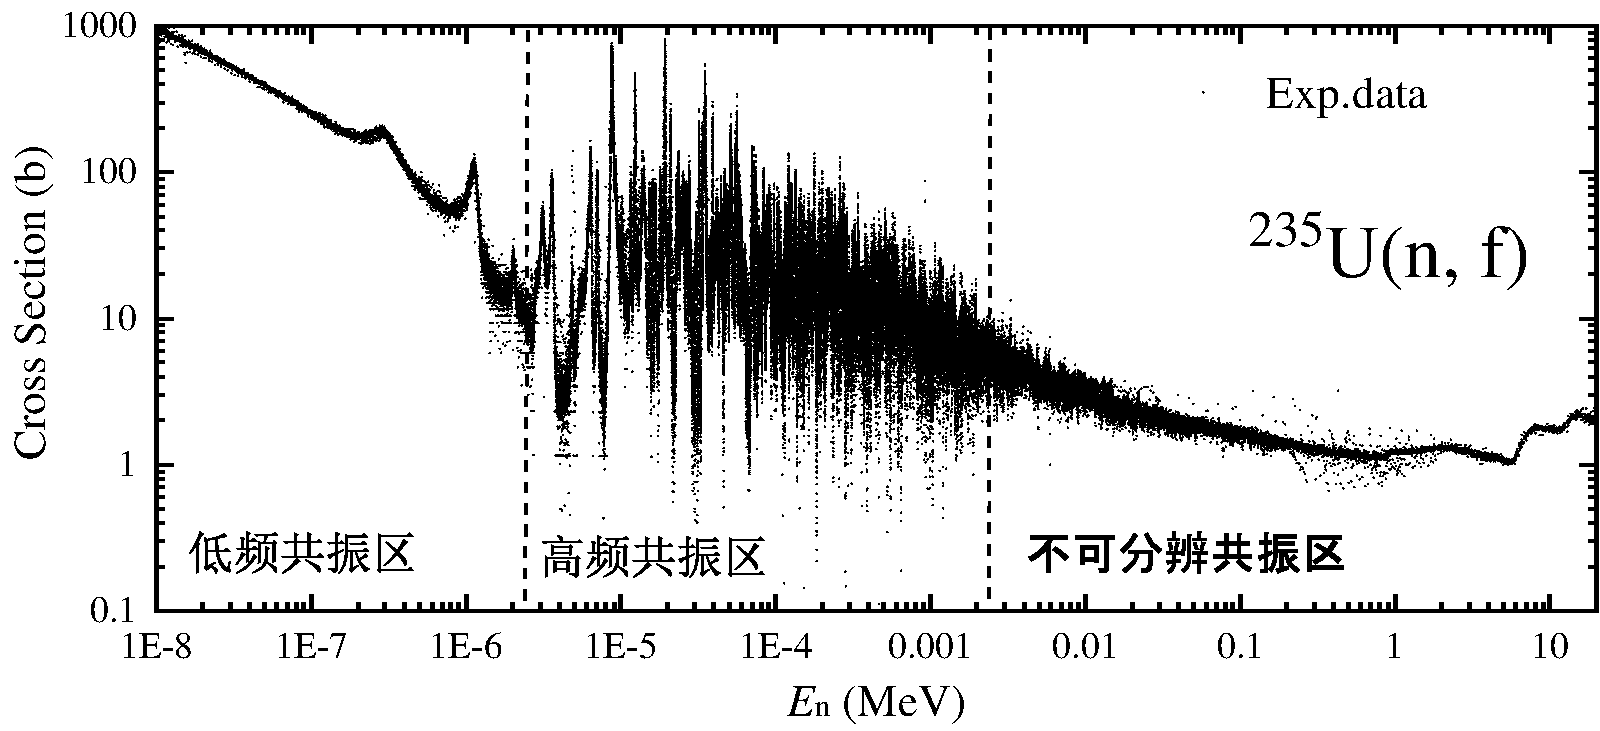
\includegraphics[width=0.9\linewidth]{figures/U235exp.pdf}
  \caption{$^{235}\text{U}(n,f)$反应截面数据}
  \label{u235expendf}
\end{figure}

实验表明:除氕、氘、氚以外的所有核素均存在中子共振现象,但不同核素的共振谱各不相同,每种核素都有其独一无二的中子共振谱。中子共振截面具有几大鲜明的特征\cite{庹先国2020中重核中子共振研究及应用进展}:1)特定核素的峰值出现在特定的能量下,这一性质为同位素识别、同位素定量测量以及它们衍生的各类核探测技术提供了强有力的支撑。2)中子共振截面非常大,常常高于快中子能区几个数量级,这在实际应用中非常重要并产生极大的影响。3)中子共振截面不受压力、温度、湿度、形状、大小等物质形态的影响。中子共振截面因具备上述特性,可应用于多种极端条件,如炸药爆轰或冲击波等动态系统中最难测量的瞬时温度;无损检测极其珍贵稀缺文物、涡轮叶片、航空发动机等特定核素的含量和分布;核反应堆中铀富集度检测或二氧化钚分布检测;发生融堆核事故后核燃料形态和新核素形成检测等。

每个峰的最高点对应的激发能被称为共振能量或共振能级,每个峰对应的半宽度是共振宽度。共振截面、共振能量和共振宽度是描述中子共振现象的基本物理量,这些用于描述中子与原子核间相互作用中的共振现象的物理量又称为共振参数,共振参数主要包含以下几个物理量:
% 共振截面、共振能量、共振宽度、共振能级自旋宇称
\begin{enumerate}[(1)]
  \item 共振截面。共振截面是指粒子在通过物质时,发生特定频率的共振吸收的概率。在核物理领域,共振截面通常指中子与原子核相互作用时,发生裂变反应的截面。中子与原子核相互作用会导致中子在原子核内部不断反弹,当中子的能量和原子核的固有能量匹配时,就会发生共振吸收并引起裂变反应。这个匹配能量对应的中子能量就是共振能,对应的共振截面就是中子能量等于共振能时的截面。
	\item 共振能量。中子共振能量是指中子与原子核之间相互作用发生共振时的能量\cite{cierjacks1980high}。中子与原子核相互作用时,复合核会形成一些离散的能级,这些能级与原子核结构有关。中子共振能量的测量可以通过中子散射实验或共振吸收实验来获得。中子散射实验通常是将一束中子入射到样品上,然后测量散射角度和能量分布等参数,通过分析实验数据得到中子共振能量。共振吸收实验是通过测量材料对中子束的吸收率来获得中子共振能量。
	\item 共振宽度。中子共振宽度描述了共振态能量附近反应截面的变化范围。共振宽度反映了共振态的寿命,即共振态存在的时间长短。根据反应道的类型,共振宽度可以分为总宽度、光子辐射宽度,中子宽度,质子宽度等几种类型。总宽度是指所有粒子通道的总和,包括弹性和非弹性散射以及各种反应产物。光子辐射宽度表示发射$\gamma$光子的能级宽度,中子宽度表示发射中子的宽度,质子宽度表示发射质子的宽度。
    \item 自旋宇称。中子共振自旋是指中子与原子核相互作用形成的共振态所具有的自旋角动量\cite{hore2015nuclear}。核子是费米子,费米子的自旋通常用半整数表示,例如1/2等。中子共振自旋对于核反应的选择规律和谱线结构有着重要影响。中子共振中宇称是指中子与原子核相互作用形成的共振态所具有的宇称量子数。宇称通常用正负号表示,分别表示偶宇称和奇宇称。中子共振宇称对于核反应的对称性和选择规律有着重要影响。
\end{enumerate}

中子共振参数在核反应相关领域有着广泛的应用。中子共振参数可以用于预测核反应截面\cite{seidl1949interpretation},这对于新一代核能技术,基础核物理学,国防战略武器研究\cite{郭之虞2003核技术及其应用的发展}中起着重要作用。
% 核能领域的设计和安全评估非常重要。此外,中子共振参数还可以用于辐照损伤的研究,以及用于确定放射性同位素的衰变方式和速率等。
总之,中子共振参数是研究核反应机制和核结构的重要物理参数,具有广泛的应用前景。通过不断深入研究和应用,可以更好地掌握核反应的规律性和特征,为核能领域的应用提供更好的理论支持和技术保障。

要得到精准的共振核数据,一个关键性的前提条件就是要能拟合好这些高频振荡的截面数据,这个问题在我国一直没有得到很好的解决。
% 但是,在实际应用中,我们用的更多的是共振参数。
目前,能拟合这些高频振荡的截面数据并得到共振参数的方法有R矩阵方法\cite{descouvemont2010r},核反应R矩阵理论是研究中重核核反应中共振能区核反应的重要理论方法。在国际上有很多程序都可以用R矩阵方法来计算中子共振,美国橡树岭国家实验室早在上世纪七十年代就组建团队,并于1980年研制出大型SAMMY程序\cite{larson1998updated}用于中子共振核数据的评价工作,其后不断改进和更新多种版本。SAMMY程序在美国各重要单位(如ORNL\cite{bell1973origen}、KAPL、LANL\cite{ren2000recent}、TUNL\cite{kelley2004tunl}等)及很多国家(如比利时、日本、法国、保加利亚等)得到广泛应用,但该程序的最新版本在我国并未得到授权使用。在国内,清华大学陈振鹏教授等人曾先后耗时三十余年发展了RAC模型\cite{chen1990r}、中国核数据中心及南开大学蔡崇海教授组成联合团队在最近10年发展了FDRR模型\cite{ge2020cendl}。两团队各自取得显著进展,能给出一定的结构信息,并成功应用于中子诱发$^6$Li、$^7$Li和$^9$Be等几个轻核反应\cite{陶曦201520},只是这些轻核反应的中子共振峰仅有1个或很少几个。受理论模型及计算方法局限,如要推广到几十至几百个共振峰、入射能区达几个数量级、从轻核到重核较大范围靶核体系,RAC和FDRR模型与SAMMY-8仍有较大差距。
% 于是,本文尝试使用机器学习方法学习这些高频振荡的截面。


\section{机器学习方法在核物理中的应用}
随着实验核物理与核理论的发展,中子共振数据的种类和数量越来越多。在国内,有CSNS反角白光中子源\cite{唐靖宇2020白光中子源及其多学科应用}获得的最新各类中子共振截面\cite{张奇玮2021基于}。而机器学习方法恰好依赖这些大数据。目前机器学习方法在核物理领域的各个领域均得到了广泛应用\cite{boehnlein2022colloquium,李庆峰2022机器学习在原子核物理中的应用专题},例如核理论、核实验、核数据和加速器等领域。

在核理论领域,可使用深度神经网络、贝叶斯神经网络\cite{樊春玲2009贝叶斯神经网络建模预测方法及其应用}和基于决策树的模型来预测原子核的各种性质,如核质量\cite{Niu2018}、电荷半径\cite{shang2022prediction}、 $\alpha$衰变半衰期\cite{saxena2021modified}、 $\beta$衰变半衰期\cite{minato2022calculation,niu2019comparative}、核裂变碎片质量分布\cite{wang2021optimizing}、核聚变截面\cite{Akkoyun2020}等。

在低能核物理领域,可使用机器学习表示原子核的变分波函数,解决“从头计算”方法中的维数灾难问题。还可使用贝叶斯神经网络确定核能量密度泛函中的参数及其不确定度,评估快中子的捕获过程、致密核物质状态方程以及中子星质量半径关系中的不确定性。

在高能核物理领域,可使用贝叶斯分析从高能重离子碰撞数据中提取夸克胶子等离子体 QGP 的性质和相图信息\cite{庞龙刚2020深度学习在核物理中的应用}。还可使用生成对抗网络(GAN)和流模型 (flow-based model) 产生格点量子色动力学 Lattice QCD 的组态(configurations),并使用深度神经网络表示 QGP 中重味夸克反夸克之间的相互作用势能 V ,可数值求解薛定谔方程。

在实验核物理、加速器设计和核数据领域,可使用聚类做反常探测,自动标注出现问题的谐振腔。还可使用强化学习\cite{wiering2012reinforcement}优化加速器中多个组件的配合。

中子共振作为核物理学中的一个重要研究领域。使用机器学习算法,可以加速计算和提高计算精度,帮助研究人员更深入地了解中子共振现象和物理机制。



总之,机器学习为中子共振研究提供新的思路和方法,加速计算、提高计算精度、进行数据分析和拟合物理模型。随着机器学习算法的不断发展和优化,它将在中子共振研究领域中发挥越来越重要的作用。




% 核反应的共振现象是指在能量较低的核反应中,由于入射粒子的质心系动能与入射粒子和靶核的结合能恰好等于复合核能级的一个能量产生的现象。共振参数是描述核反应共振现象的重要参数,包括共振能量、共振宽度和共振强度等。

% 在核反应研究领域,预测和解析共振参数是一个具有挑战性的问题。传统的理论模型虽然能够描述核反应的基本物理过程,但是面对实验数据中的复杂性和不确定性,预测精度和可靠性往往难以满足实际需求。

% 随着计算机技术和机器学习方法的不断发展,越来越多的研究人员开始尝试使用机器学习方法来预测和解析核反应的共振参数。机器学习方法能够从大量数据中自动学习规律和模式,对于核反应研究来说,这意味着我们可以从大量实验数据中提取共振参数的信息,并用于预测未知的反应过程。与传统的理论模型相比,机器学习方法可以更好地处理实验数据中的复杂性和不确定性,从而提高预测精度和可靠性。



% 新一代核能技术、核天体物理、基础核物理学、核医学和国防战略武器研究\cite{郭之虞2003核技术及其应用的发展}等,对中子共振核数据在精度、入射能区、靶核范围有较强烈的需求。美国橡树岭国家实验室早在上世纪七十年代就组建团队,并于1980年研制出大型SAMMY程序\cite{larson1998updated}用于中子共振核数据的评价工作,其后不断改进和更新多种版本。SAMMY程序在美国各重要单位(如ORNL\cite{bell1973origen}、KAPL、LANL\cite{ren2000recent}、TUNL\cite{kelley2004tunl}等)及很多国家(如比利时、日本、法国、保加利亚等)得到广泛应用,但由于“众所周知”原因,我国一直没能得到授权使用。随着我国相继在中子共振核数据的投入及取得的进展,美国最近才公开了其2008年的版本(SAMMY-8),以此消耗我国在中子共振领域的持续研究。清华大学陈振鹏教授等人曾先后耗时三十余年发展了RAC模型\cite{chen1990r}、中国核数据中心及南开大学蔡崇海教授组成联合团队在最近10年发展了FDRR模型\cite{ge2020cendl}。两团队各自取得显著进展,能给出一定的结构信息,并成功应用于中子诱发$^6$Li、$^7$Li和$^9$Be等几个轻核反应\cite{陶曦201520},只是这些轻核反应的中子共振峰仅有1个或很少几个。受理论模型及计算方法局限,如要推广到几十至几百个共振峰、入射能区达几个数量级、从轻核到重核较大范围靶核体系,RAC和FDRR模型与SAMMY-8仍有较大差距。针对此种现状,本项目引入人工智能方法,首先构建可适用于低频变化的中子核数据的深度神经网络模型(DNN),以此探讨DNN模型在核数据领域中应用的可行性。在此基础上,融合R-矩阵理论和弹靶合成复合核的结构特征量,依托,借鉴平行相移理论(PPS),构建能同时适用于低频和高频变化的中子共振核数据的平行相移深度神经网络模型(PPSDNN),研究具有自主知识版权、入射能区广、靶核适用范围宽的中子共振核数据分析方法和评价系统,同时给出理论预言值误差范围,实现我国在中子共振核数据评价领域的“弯道超车”。
本文将基于机器学习方法对核反应的共振现象展开研究。
% 我选择的机器学习算法是平行相移深度神经网络——PPSDNN(Parallel Phase Shift Deep Neural Network)。
本文安排如下:在引言中,介绍了
% 核反应的基本物理过程和共振参数的定义,然后介绍机器学习方法在核反应研究中的应用,
什么是机器学习和中子共振数据,
以及机器学习在核物理中的应用。在第二章中,先介绍机器学习中最常用的深度神经网络(DNN)算法,然后引出DNN模型及频率原则(f-principle)。接着详细介绍所采用的机器学习算法和模型——PPSDNN模型,并给出算法流程。在第三章中,首先给出PPSDNN模型在玩具模型(toy model)中的测试结果。接着介绍PPSDNN在学习中子共振数据中的应用。最后,在第四章中,先对以上内容作出总结,接着介绍机器学习用于中子共振研究的潜在应用及其和R-Matrix模型相结合的可能性,给出展望。


